\section{Project management}

% Include a timetable (in 2 week chunks) for the remainder of the academic year, up until the submission deadline.

\subsection{The Updated Timeline}
Although the project is on track to meet the schedule set out in the specification, alterations to the schedule have been made. The most major change stems from the realisation that the generation and radio message processing systems can be developed simultaneously, and make sense to be developed in this way. Therefore these two activities have been extended until mid December and been recorded as simultaneous. This has pushed back other tasks, but after researching speech input and taking into account the simple approach decided on, this task has been shortened in duration. Ensuring compliance with the CAP413 manual has also been reduced in duration, given that this will be a brief pass looking over the system's responses and checking them against the manual. Full compliance is was not a stated requirement of the system. The evaluation day has also been marked on the schedule, which will involve getting user feedback from technical users unfamiliar with the project. This feedback can be used to make improvements but these will be made during the execution of the remaining tasks so are not shown on the updated GANTT chart.

\begin{figure}[H]
    \centering
	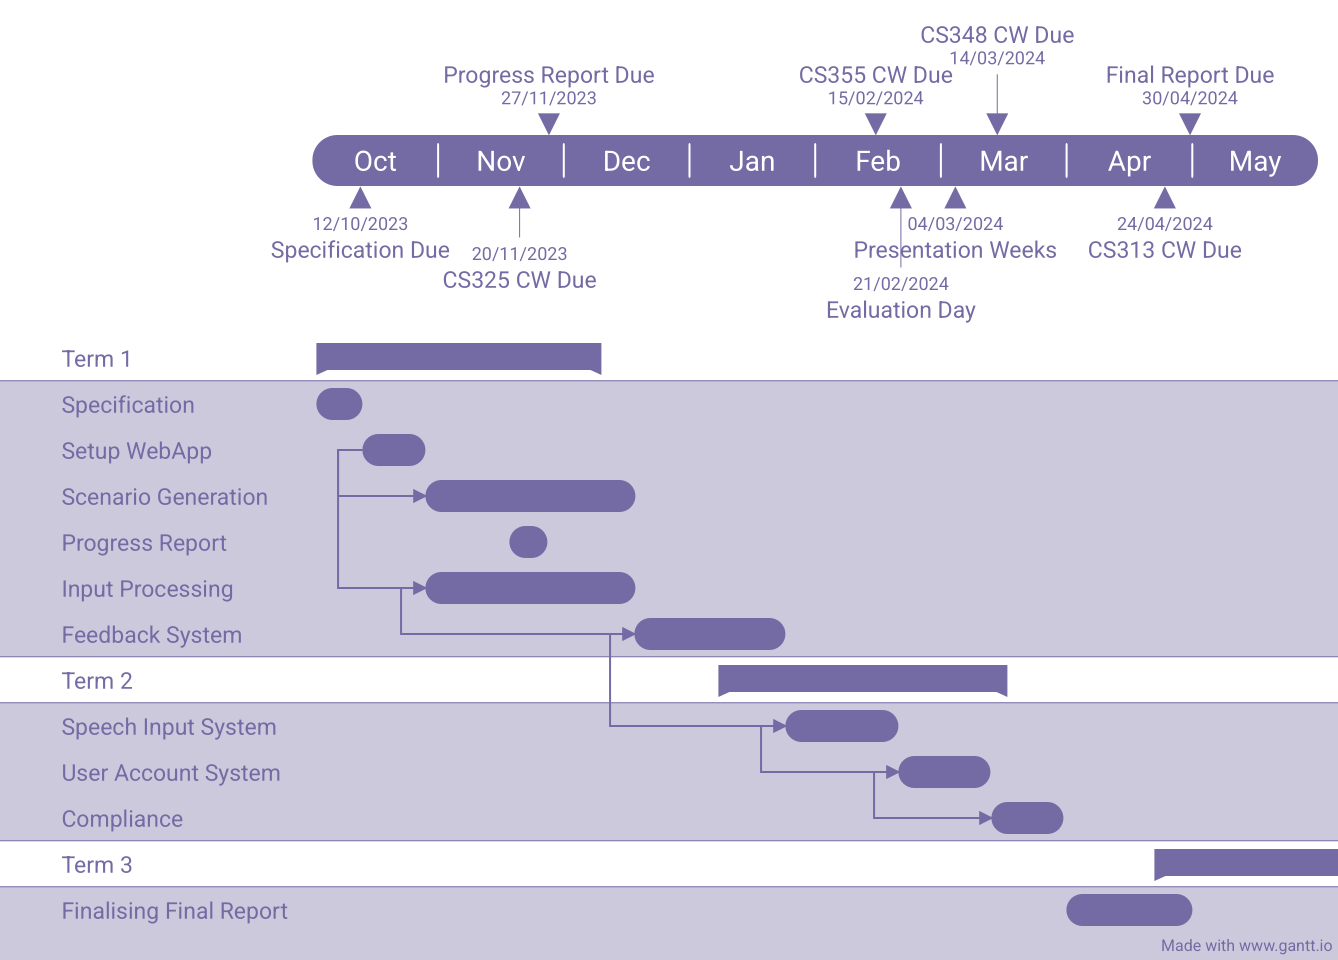
\includegraphics[scale = 0.3]{../document-resources/images/GANTT-for-Progress-Report}
    \label{progress-report-gantt}
    \caption{Current project timeline.}
\end{figure}

\subsection{Improvements to Working Methods}
No major issues have been encountered so far with the project, but a few changes to working methods will be made to ensure project success. 
\begin{itemize}
    \item More frequent communication with the client will ensure that the features required are correctly implemented once they reach a testable state. The client is the subject expert, and communication will reduce time spent on subject research.
    \item Less time will be spent trying to reinvent the wheel - if a freely available library exists which solves a problem, it should be tried before writing a new solution. Time was previously wasted on specific UI features which ended up being replaced by library code.
    \item Simple solutions will be tried before attempting to create complex solutions to reduce development time and improve maintainability. Parsing was over complicated before a simple, and correct, solution was found.
    \item Work on deliverable project documents will be started earlier than they have been so far to smooth out the workload. Two large coursework deadlines being close to one another has not been handled as well as it should have been.
\end{itemize} 